% Create a Table of Contents in Beamer
\documentclass[10pt,t]{beamer}
% Theme choice:
\usetheme{Singapore}
\usecolortheme{whale}
\setbeamercolor{titlelike}{fg=blue,bg=white}
\setbeamercolor{frametitle}{fg=blue,bg=white}
\setbeamertemplate{frametitle}[default][left]
\setbeamertemplate{navigation symbols}{}

\usepackage{graphicx}
\usepackage{amsmath}
\usepackage{amsfonts}
\usepackage{amssymb}
\usepackage{amsthm}

% Title page details: 
\title{Chapter 0: Introduction and Review} 
\author{Taylor Okonek \& Charlie Wolock}
\date{\today}



\begin{document}
	% Title page frame
	\begin{frame}
	\titlepage 
\end{frame}
% Outline frame
\begin{frame}{Outline}
\tableofcontents
\end{frame}

\AtBeginSection[ ]
{
\begin{frame}{Outline}
\tableofcontents[currentsection]
\end{frame}
}

% Presentation structure
\section{Syllabus}

\begin{frame}{Instructors}

\begin{figure}
	\begin{center}
		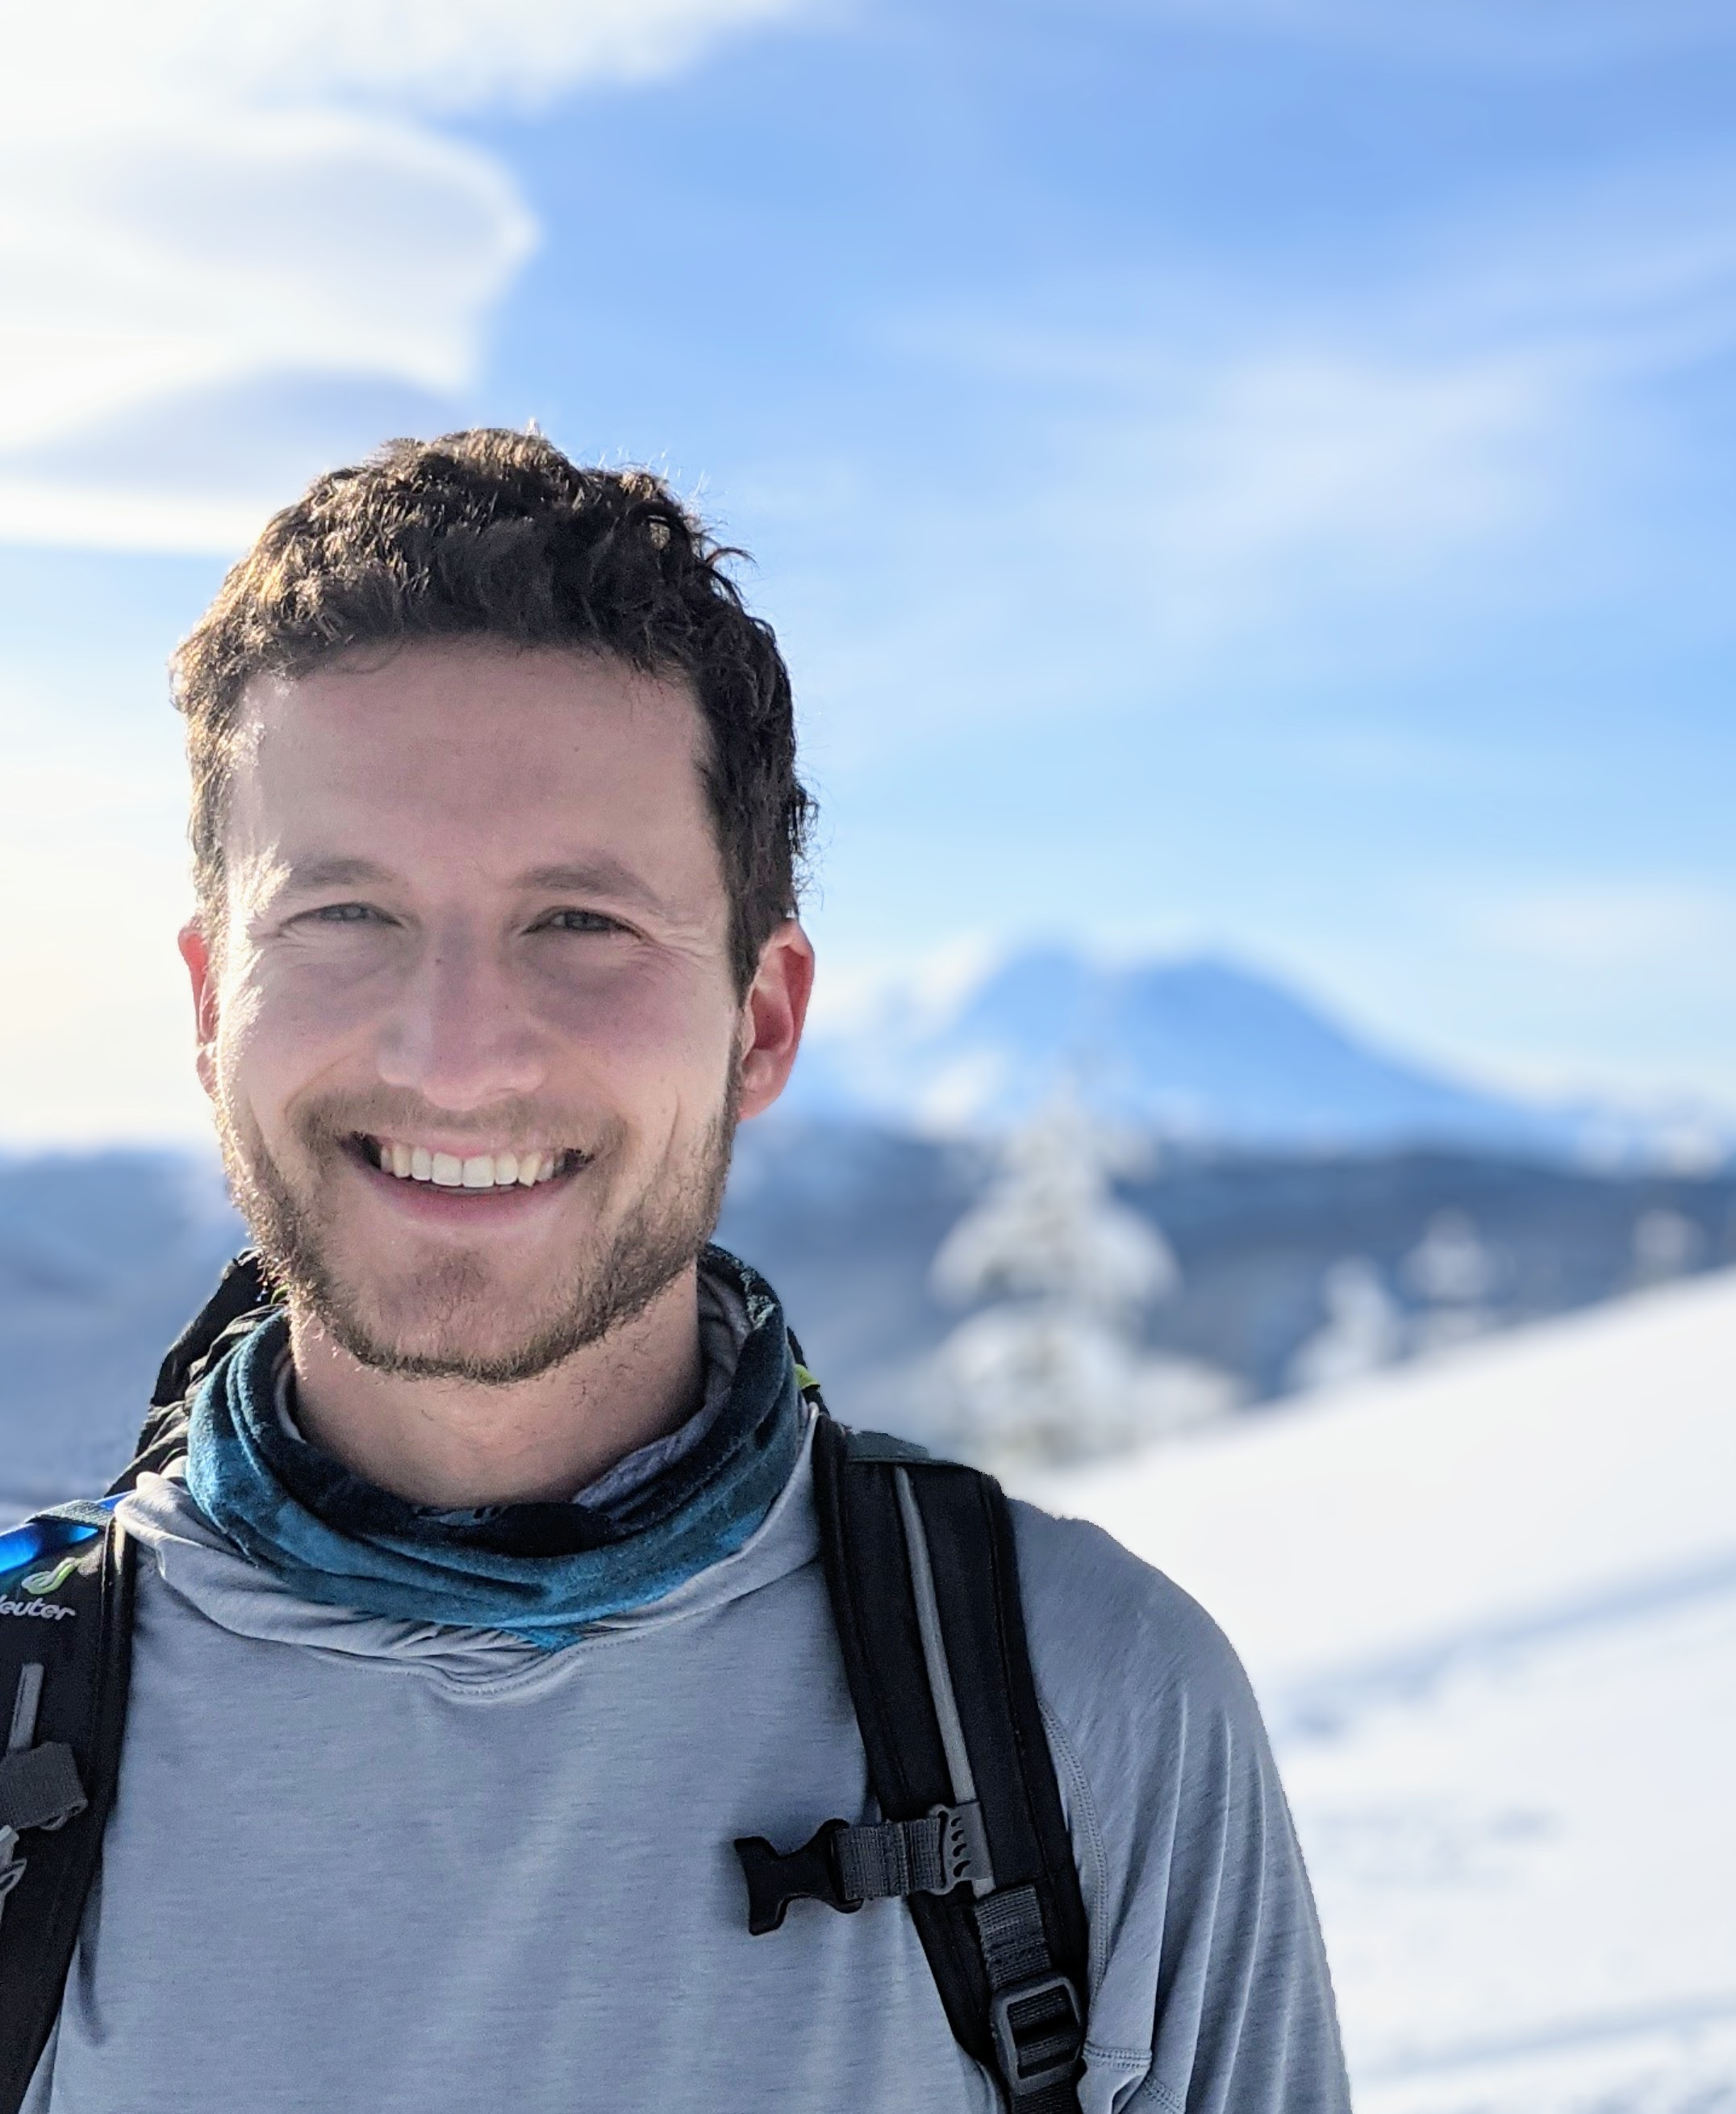
\includegraphics[height=0.4\textheight]{charlie.jpg} 
		\hspace{2cm}
		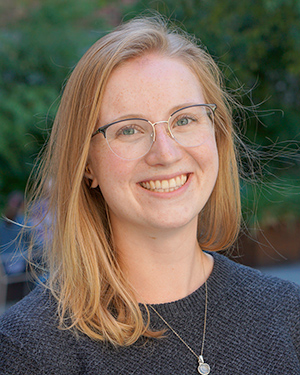
\includegraphics[height=0.4\textheight]{taylor.jpg}
	\end{center}
\end{figure}

\begin{columns}
	\begin{column}[t]{0.4\textwidth}
            \small Charlie Wolock (he/him) \\ 
            cwolock@uw.edu \\~\
            
            \small 4th year Ph.D. Student, Dept. of Biostatistics \\
            \small Statistical interests: Nonparametrics, survival analysis
	\end{column}
	\begin{column}[t]{0.4\textwidth}  %%<--- here
			\small Taylor Okonek (she/her) \\
			tokonek@uw.edu  \\~\ 
			
			\small 4th year Ph.D. Student, Dept. of Biostatistics \\
			\small Statistical interests: spatial stats, infectious disease
	\end{column}
\end{columns}

\end{frame}

\begin{frame}{Course description}
``Introduction to regression methods for analysis of continuous, binary, and time-to-event (survival) data. Covers linear regression, logistic regression, and proportional hazards regression, all at an introductory level. Makes use of examples drawn from the biomedical and health sciences literature." \\~\

\begin{itemize}
	\item Graded, 4 credits
	\item Course website: canvas.uw.edu
	\item No textbooks for the course, all material needed for homeworks/project can be found in lecture and discussion section slides
\end{itemize}

\end{frame}

\begin{frame}{Logistics}
Class sessions times and room (if not on zoom) \\
Office hours times and room (if not on zoom)
\end{frame}

\begin{frame}{Learning objectives}
\begin{itemize}
	\item Interpret numerical and graphical summaries of data that are relevant to medical and health sciences studies
	\item Interpret coefficients in linear, logistic, and proportional hazards regression models in the context of health outcomes
	\item 
Select an appropriate regression model based on a scientific question and study design
	\item Describe the necessary assumptions for linear, logistic, and proportional hazards regression in the contexts of estimation and prediction
	\item Develop and interpret confidence intervals for model parameters
	\item Set up and carry out appropriate hypothesis tests for linear, logistic, and proportional hazards regression models
	
\end{itemize}
\end{frame}

\begin{frame}{Learning objectives (continued)}
\begin{itemize}
	\item Use linear and logistic regression models to make predictions
	\item Use diagnostic procedures and sensitivity analyses to investigate potential deviations from model assumptions
	\item Use the statistical software R to:
	\begin{itemize}
		\item Read in data files
		\item Calculate summary statistics and create appropriate graphical displays
		\item Perform basic statistical inference procedures
		\item Fit linear, logistic, and proportional hazards regression models
	\end{itemize}
\end{itemize}
\end{frame}

\begin{frame}{Class communication}
We will communicate with you outside of class using the Canvas page, so please sign up to receive email notifications for the page. \\~\

Questions about course context or homework assignments should be posted to the Canvas Discussion Board, \textbf{not sent via email}. We will monitor the discussion board regularly, and also strongly encourage you to reply to each other’s questions. Concerns of a personal nature can be communicated with us via email, and in general any emails should be sent to both instructors. \\~\

Please communicate respectfully to your classmates and to us, and let us know if there are ways classroom communication can be made more accessible to you. \\~\

Instructors will not send same-day responses to messages sent after 8:00pm PST.
\end{frame}

\begin{frame}{Homework}

Homework assignments will be posted on the Canvas website one week 
prior to the due date. They should be completed in a Word or .pdf document and 
submitted electronically to the Canvas website by the due date. You are welcome to work together on homework; however, your submitted assignment (including R code, if applicable) should be in your own words. \\~\

Solution keys and individual feedback will be provided. \textcolor{red}{We have prepared a guide for how to present your assignments which is available on our Canvas page.} The lowest homework score will be dropped.

\end{frame}

\begin{frame}{Homework: Late policy}
Throughout the quarter, you may use up to three homework 
extension days. These three days may be divided up for homework assignments however you choose (for example: all three days for a single assignment, one day each for three separate assignments). \\~\

In order to use your extension days, \textbf{you must email both instructors prior to the homework due date} to inform them you plan to use an extension day. If you do not email the instructors prior to homework due date, the extension days will not be counted, and your homework will be counted as late. \\~\

Late homework receives no credit.

\end{frame}

\begin{frame}{Quizzes}
There will be weekly, open-note Canvas quizzes on Mondays. These quizzes are designed to ensure that you keep up with course material and can recall material from previous weeks. Each quiz will consist of 10 questions, 3 of which will be on information from previous weeks, and 7 of which will be on material from the most recent week of lectures. Questions will be a mix of multiple choice, True/False, and open response. \\~\

Quizzes will be graded Monday evening, and you will have 48 hours from Monday 11:59pm PST to Wednesday 11:59pm PST to complete quiz revisions, for the opportunity to earn back up to 50\% of the points you missed.
\end{frame}


\begin{frame}{Discussion section}
Discussion sections will consist of \textcolor{red}{group activities}, review of class material, discussion of group projects, and practice using R. You will be required to hand in a brief exercise (credit/no credit) at each discussion section. Your discussion section score will be based on completion of these assignments. To receive full credit for discussion section, you can miss at most one of the discussions.
\end{frame}

\begin{frame}{Final Project}
There will be a final data analysis project for which you will be given a dataset (or select your own, with approval from the instructors) and asked to develop a appropriate analysis plan, carry out the analysis, and write a short report. Projects will be introduced in the first discussion section. \textcolor{red}{You will complete your project in small groups, assigned by the instructors.}
\end{frame}

\begin{frame}{Grading}
\begin{columns}
	\begin{column}[t]{0.4\textwidth}
		Homework \\
		Quizzes \\
		Final Project \\
		Discussion Section 
	\end{column}
	\begin{column}[t]{0.4\textwidth}  %%<--- here
		30\% \\
		30\% \\
		30\% \\
		10\% 
	\end{column}
\end{columns}

\vspace{1cm}

At the end of the course, we will convert your percentage to the UW 0.0-4.0 scale. Final course grades will be calculated based on the guidelines linked below. At minimum, you will get an A (3.9-4.0) if you earn at least 95\% of the total possible points, an A- (3.5-3.8) if you earn between 90\% and 95\% of the total possible points, and a C- (1.5-1.8) if you earn 65\% of the total possible points. \\~\

Guidelines: http://depts.washington.edu/grading/practices/guidelines.html 

\end{frame}

\begin{frame}{Course policies}
\begin{itemize}
	\item \textbf{Laptops}: You will be expected to have access to a laptop during discussion sections. However, you will not generally need access to a computer during lecture (different if zoom, obviously).
	\item \textbf{Computing}: Computing in R is an important component of this course. FIND OUT WHERE THEY CAN BORROW COMPUTERS and include here. Please see us if this expectation will cause trouble for you, and we can work out a solution.
\end{itemize}
\end{frame}

\begin{frame}{Course policies (continued)}
\begin{itemize}
	\item \textbf{Collaboration}: You are encouraged to work together on homework assignments, but the final write-up should be done individually. The course project will be a \textcolor{red}{group project}; you will discuss approaches to the project with your group and other classmates during discussion sections, but outside of class you may only discuss your project with your group members and the instructors.
	\item \textbf{Academic Honesty}: Students are encouraged to familiarize themselves with the academic honesty policies. If you hand in work that is not written in your own words, you will at minimum lose all credit for the problem, and at maximum all credit for the assignment. Issues surrounding academic integrity will be handled in accordance with university policies.
\end{itemize}
\end{frame}

\begin{frame}{Course policies (continued)}
\begin{itemize}
	\item \textbf{Grading}: We will have assignments graded in a timely fashion. If you have questions or concerns about the grading, see us. We reserve the right to change or not change the grade.
\end{itemize}
\end{frame}

\begin{frame}{Classroom climate}
The UW School of Public Health seeks to ensure all students are fully included in each course. We strive to create an environment that reflects community and mutual caring. We encourage students with concerns about classroom climate to talk to your instructor, your advisor, a member of the departmental or SPH Diversity Committee and/or the program director. DCinfo@uw.edu is a resource for students with classroom climate concerns.
\end{frame}

\begin{frame}{Concerns}
If you have any concerns about the class or your instructors, please feel free to talk to or email us at any time during the quarter. If you are not comfortable talking with us or not satisfied with the response that you receive, you may contact the Department of Biostatistics Associate Director of Academic Affairs (biostgp@uw.edu). If you still are not satisfied with the response, you may contact the Department of Biostatistics Chair (bchair@uw.edu). You may also contact the Graduate School at G-1 Communications Building, by phone at 206-543-5139 or by email at raan@uw.edu.
\end{frame}

\begin{frame}{Academic integrity}
Students at the University of Washington (UW) are expected to maintain the highest standards of academic conduct, professional honesty, and personal integrity.
 \\~\

The UW School of Public Health (SPH) is committed to upholding standards of academic integrity consistent with the academic and professional communities of which it is a part. Plagiarism, cheating, and other misconduct are serious violations of the University of Washington Student Conduct Code (WAC 478-121). We expect you to know and follow the university’s policies on cheating and plagiarism, and the SPH Academic Integrity Policy. Any suspected cases of academic misconduct will be handled according to University of Washington regulations. For more information, see the University of Washington Community Standards and Student Conduct website.

\end{frame}

\begin{frame}{Access and accommodation}
\small Your experience in this class is important to us. If you have already established accommodations with Disability Resources for Students (DRS), please communicate your approved accommodations to us at your earliest convenience so we can discuss your needs in this course.
\\~\

\small If you have not yet established services through DRS, but have a temporary health condition or permanent disability that requires accommodations (conditions include but not limited to; mental health, attention-related, learning, vision, hearing, physical or health impacts), you are welcome to contact DRS at 206-543- 8924 or uwdrs@uw.edu or disability.uw.edu. DRS offers resources and coordinates reasonable accommodations for students with disabilities and/or temporary health conditions. Reasonable accommodations are established through an interactive process between you, your instructor(s) and DRS. It is the policy and practice of the University of Washington to create inclusive and accessible learning environments consistent with federal and state law.

\end{frame}

\begin{frame}{First Canvas quiz!}
Please complete the Canvas quiz by Friday! \textcolor{red}{tbd a bit, but we should do something like this probably} 

\vspace{0.3cm}

\begin{itemize}
	\item Name
	\item Pronunciation guide
	\item What are you most looking forward to learning this quarter?
	\item What do you anticipate having the most trouble with this quarter?
\end{itemize}

\vspace{0.3cm}

Pronunciation guide example:
\begin{itemize}
	\item Taylor Okonek
	\item TAY-lor AH-ke-nik
\end{itemize}

\vspace{0.3cm}

\color{blue} We'll do a mid-quarter Stop/Start/Continue check-in as well!

\end{frame}

\begin{frame}{What to Expect: Statistics}
You will need light algebra and mathematical reasoning
\vspace{0.3cm}
\begin{itemize}
	\item No calculus assumed
	\item We won't prove technical results, but can provide resources for those available if asked
	\item Quizzes will not require any math beyond basic arithmetic, and are open note
\end{itemize}

\vspace{0.3cm}

This course is the natural sequel to BIOST 310 

\vspace{0.3cm}

We will learn how to build regression models, estimate parameters, and interpret coefficients 

\vspace{0.3cm}

Examples will be primarily in public health or health sciences applications

\end{frame}

\begin{frame}{What to Expect: Computing}
We will learn basic statistical computing in \texttt{R}

\vspace{0.3cm}

You are \textit{not} expected to have a computing background

\vspace{0.3cm}

\begin{itemize}
	\item We will demonstrate important functions in lectures and discussion sections
	\item We will provide helpful resources: templates for homework assignments, \texttt{R} code "cheat sheets" with useful functions, video tutorials (as applicable), etc. \textcolor{red}{We need to make cheat sheets i guess}
\end{itemize}

\vspace{0.3cm}

\textbf{Homework for tonight:} download \texttt{R} and \texttt{R Studio} (see instructions on Canvas) \textcolor{red}{need to make instructions}

\end{frame}

\begin{frame}[c]
\centering \huge Any Questions?
\end{frame}

\section{Motivation}

\begin{frame}{Why is statistics important?}
\begin{itemize}
	\item We have a research question we want to answer
	\item We hear a claim we think is false, and want to refute it
	\item We have a \textit{ton} of information and we don't know how to make sense of it
	\item We understand the current state of things, but want to predict future outcomes
\end{itemize}
\end{frame}

\begin{frame}{Example: Research question}

Retinol (a Vitamin A derivative) is a popular skin care agent that has been shown in studies to decrease wrinkle surface area and hyperpigmentation. However, retinol is not safe to use for pregant individuals, and additionally retinol has known side-effects of causing skin dryness and stinging for many people. Bakuchiol has been proposed as a retinol alternative that is safe for pregnant individuals to use and does not have similar negative side-effects. However, we are not sure if Bakuchiol is \textit{as effective} as retinol for decreasing wrinkle surface area and hyperpigmentation. 

\vspace{0.3cm}

Q: \textit{Is Bakuchiol as effective as retinol for improving wrinkle surface area and hyperpigmentation?} 

\vspace{0.3cm}

How do we answer this question? (one option: \href{https://onlinelibrary.wiley.com/doi/10.1111/bjd.16918}{a randomized trial})

\end{frame}

\begin{frame}{Example: Research question}

\begin{itemize}
	\item Randomly assign 44 individuals to either use Bakuchiol or Retinol over the course of 12 weeks, surveying individuals and taking images every 4 weeks 
	\item Use image analysis to determine fine wrinkle surface area at each time point
\end{itemize}

\centering 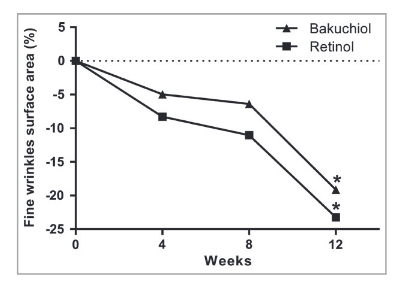
\includegraphics[scale=0.4]{retinol.png}

\end{frame}

\begin{frame}{Example: Research question}

Why is statistics important?

\vspace{0.3cm}

In this example:
\begin{itemize}
	\item Allows us to determine whether or not there is a difference in outcomes based on exposure (retinol vs. Bakuchiol) that is due to \textit{the exposure alone} (i.e. no other variable could have mattered)
	\item A standardized way of measuring the outcome. This study didn't compare qualitatively if they thought individuals had a lower wrinkle surface area, they used image analysis!
	\item Allows us to determine if there is a \textit{statistically significant} difference in outcomes between Bakuchiol and retinol users (we'll come back to this throughout the course)
\end{itemize}

\end{frame}

\begin{frame}[c]{Example: Refuting a false claim}
\centering 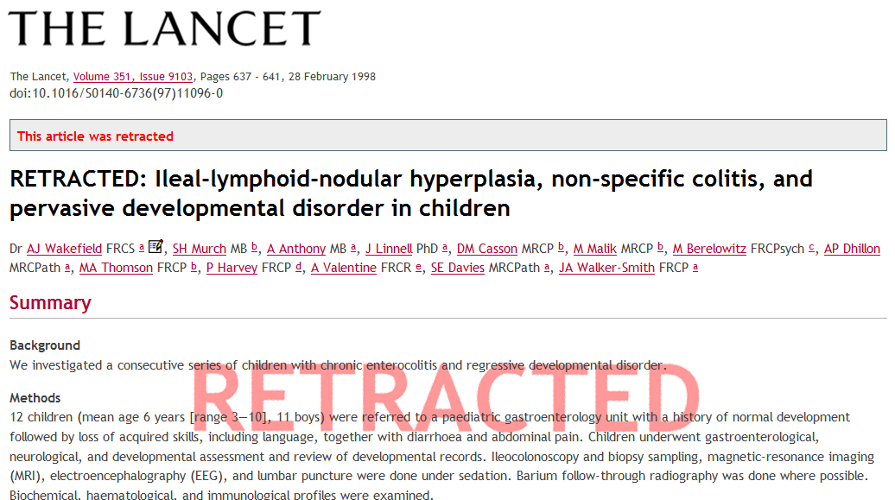
\includegraphics[scale=0.4]{lancet.png}
\end{frame}

\begin{frame}{Example: Refuting a false claim}
A paper published in the Lacet (a relatively high-impact journal!) in 1998 suggested that the measles, mumps, and rubella (MMR) vaccine may cause autism spectrum disorder in children.

\centering 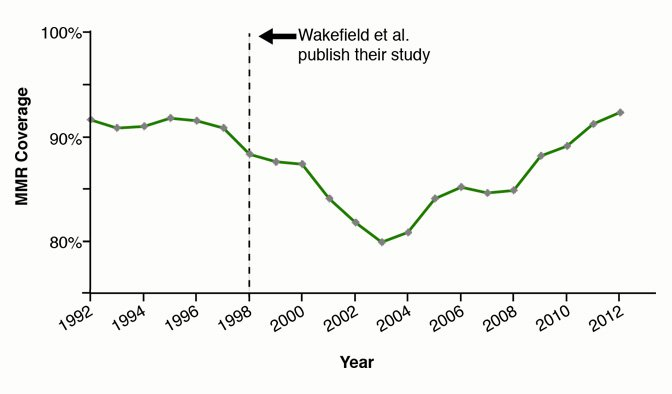
\includegraphics[scale=0.4]{mmrvax.jpg}

\end{frame}

\begin{frame}{Example: Refuting a false claim}

Statistical tools used to critically assess (and eventually refute) this claim:
\begin{itemize}
	\item The sample size in their study was $n = 12$ (which is \textit{very} small)
	\item Their study design was uncontrolled, so causal claims could not be made (more on this to follow in the Study Design review section!)
\end{itemize}

\vspace{0.3cm}

Why is statistics important?
\begin{itemize}
	\item Allows us to critically assess scientific claims
	\item Understanding the assumptions underlying statistical methods and study designs lets us think \textit{scientifically and statistically} about whether or not these assumptions are met
\end{itemize}

\vspace{0.3cm}

\footnotesize An important aside with this study is that the lead author was funded by lawyers who had been representing parents in lawsuits against vaccine-producing companies. Critically reading studies from \textit{many} angles (not only statistical) is important! A more detailed summary of this article and follow-up can be found \href{https://www.ncbi.nlm.nih.gov/pmc/articles/PMC3136032/}{\color{cyan} here}.

\end{frame}

\section{Study Design}

\begin{frame}{Study Design}
\textit{How you collect data impacts what questions you can (cannot) answer, what statistical methods you can (cannot) use, and what conclusions you can (cannot) draw.} \\~\

\textcolor{blue}{Extreme Example:} Suppose I'm interested in understanding public opinion about biostatistics. I randomly select on individual from our class and ask if they like biostatistics.

\begin{itemize}
	\item What questions can I answer using these data?
	\item What statistical methods can I use to analyze these data?
	\item What conclusions can I draw using these data?
\end{itemize}
\end{frame}

\begin{frame}{Experimental vs. Observational Studies}

\textcolor{blue}{Experimental:} exposure/treatment is \textit{controlled} by the researcher (e.g., randomly assign people to drug or placebo)
\begin{itemize}
	\item Randomized controlled trial 
\end{itemize}

\vspace{0.3cm}

\textcolor{blue}{Observational:} exposure/treatment is \textit{not controlled} by the researcher (e.g., we look at a group of people and \textit{observe} who smokes and who doesn't smoke)
\begin{itemize}
	\item Cross-sectional study
	\item Cohort study
	\item Case-control study
\end{itemize}
\end{frame}
	
	
\begin{frame}{Experimental vs. Observational Studies}
In \textit{experimental} studies, we can talk about \color{blue} \textit{causation}\color{black}. In \textit{observational} studies we  talk instead about \color{blue} \textit{association} \color{black}(because we worry about \color{blue} \textit{confounding}\color{black}). \\

\vspace{0.3cm}

% we'll come back to this when we talk about interpreting results
A \textit{\textcolor{blue}{confounder}} is a variable that is \textcolor{red}{causally associated EDIT I don't like this phrase} with our outcome and also associated with the exposure in our sample.  \\

\vspace{0.3cm}

\begin{itemize}
	\item[] \textit{Example:} suppose we're interested in the relationship between smoking and lung function in kids. We know that age is causally associated with lung function: as children grow and develop, their lung function improves. If age is also associated with smoking in our sample (e.g., if older kids are more likely to smoke), then age is a confounder.
\end{itemize} 

\vspace{0.3cm}

\small \textit{Much more on the topic of confounding to come...} 
\end{frame}

\subsection{Experimental studies}

\begin{frame}{Randomized controlled trial}
Description:
\begin{itemize}
	\item Take a sample from the population and \textbf{randomly assign} individuals to either treatment (\textit{exposed}) or control/placebo (\textit{unexposed}), and follow individuals to observe a specific outcome (e.g., death yes/no, disease yes/no, time to death, change in cholesterol level, \dots)
\end{itemize}
\end{frame}

\begin{frame}{Randomized controlled trial}
Description:
\begin{itemize}
	\item Take a sample from the population and \textbf{randomly assign} individuals to either treatment (\textit{exposed}) or control/placebo (\textit{unexposed}), and follow individuals to observe a specific outcome (e.g., death yes/no, disease yes/no, time to death, change in cholesterol level, \dots)
\end{itemize}
Pros:
\begin{itemize}
	\item With a large enough sample, no confounding
	\item Gold standard for establishing causality
\end{itemize}
\end{frame}

\begin{frame}{Randomized controlled trial}
Description:
\begin{itemize}
	\item Take a sample from the population and \textbf{randomly assign} individuals to either treatment (\textit{exposed}) or control/placebo (\textit{unexposed}), and follow individuals to observe a specific outcome (e.g., death yes/no, disease yes/no, time to death, change in cholesterol level, \dots)
\end{itemize}
Pros:
\begin{itemize}
	\item With a large enough sample, no confounding
	\item Gold standard for establishing causality
\end{itemize}
Cons:
\begin{itemize}
	\item Often very expensive
	\item Not always possible or ethical to randomize individuals
	\begin{itemize}
		\item Cannot randomly assign someone to a specific age, genetic variant, etc.
		\item Unethical to randomly assign harmful exposures (e.g., smoking)
	\end{itemize}
\end{itemize}
\end{frame}

\begin{frame}[c]{Randomized controlled trial}
Examples: 

\vspace{0.3cm}

\begin{itemize}
	\item \href{https://jamanetwork.com/journals/jama/article-abstract/2613159}{\color{cyan} Effect of Vitamin D and Calcium Supplementation on Cancer Incidence in Older Women}
	\item \href{http://stroke.ahajournals.org/content/36/8/1764.short}{\color{cyan} Daily Functioning and Quality of Life in a Randomized Controlled Trial of Therapeutic Exercise for Subacute Stroke Survivors}
\end{itemize}
\textcolor{red}{maybe update the second link, it's from 2005} 
\end{frame}


\subsection{Observational studies}

\begin{frame}{Cross-sectional study}
Description:
\begin{itemize}
	\item Randomly sample individuals, record their exposure and outcome at a \textit{single time point/interval} (no follow-up)
\end{itemize}
\end{frame}

\begin{frame}{Cross-sectional study}
Description:
\begin{itemize}
	\item Randomly sample individuals, record their exposure and outcome at a \textit{single time point/interval} (no follow-up)
\end{itemize}
Pros:
\begin{itemize}
	\item Relatively cheap and easy
	\item Can study multiple outcomes and exposures
\end{itemize}
\end{frame}

\begin{frame}{Cross-sectional study}
Description:
\begin{itemize}
	\item Randomly sample individuals, record their exposure and outcome at a \textit{single time point/interval} (no follow-up)
\end{itemize}
Pros:
\begin{itemize}
	\item Relatively cheap and easy
	\item Can study multiple outcomes and exposures
\end{itemize}
Cons:
\begin{itemize}
	\item Inefficient for rare exposure and disease 
	\item Time sequence of exposure and outcome (i.e. which came first) is not always clear
	\item Potential confounding (so no conclusions about causality)
\end{itemize}
\end{frame}

\begin{frame}[c]{Cross-sectional study}
Examples:
\vspace{0.3cm}

\begin{itemize}
	\item \href{http://ajph.aphapublications.org/doi/abs/10.2105/AJPH.78.10.1336}{\color{cyan} Job strain, work place social support, and cardiovascular disease in a random sample of the Swedish working population}
	\item \href{onlinelibrary.wiley.com/doi/10.1111/add.12623/full}{\color{cyan} Real-world effectiveness of e-cigarettes when used to aid smoking cessation}
\end{itemize}

\textcolor{red}{first one from 2011, second from 2014}

\end{frame}

\begin{frame}{Cohort study}
Description:
\begin{itemize}
	\item Sample people \textit{without the outcome of interest}, record their exposure, then \textit{follow} those individuals over time to observe the outcome
	\item Can be \textit{prospective} (sample people in present time, then follow-up) or \textit{restrospective} (sample people from a database collected in the past, and observe them through their time recorded in the database)
\end{itemize}
\end{frame}

\begin{frame}{Cohort study}
Description:
\begin{itemize}
	\item Sample people \textit{without the outcome of interest}, record their exposure, then \textit{follow} those individuals over time to observe the outcome
	\item Can be \textit{prospective} (sample people in present time, then follow-up) or \textit{restrospective} (sample people from a database collected in the past, and observe them through their time recorded in the database)
\end{itemize}
Pros:
\begin{itemize}
	\item Time sequence is known (exposure came first)
	\item Can study multiple outcomes 
\end{itemize}
\end{frame}

\begin{frame}{Cohort study}
Description:
\begin{itemize}
	\item Sample people \textit{without the outcome of interest}, record their exposure, then \textit{follow} those individuals over time to observe the outcome
	\item Can be \textit{prospective} (sample people in present time, then follow-up) or \textit{restrospective} (sample people from a database collected in the past, and observe them through their time recorded in the database)
\end{itemize}
Pros:
\begin{itemize}
	\item Time sequence is known (exposure came first)
	\item Can study multiple outcomes 
\end{itemize}
Cons:
\begin{itemize}
	\item Inefficient for rare outcomes
	\item Prospective cohort studies are often expensive and time-consuming to follow people, and there are opportunities for people to drop out
	\item Potential confounding (so no conclusions about causality)
\end{itemize}
\end{frame}

\begin{frame}[c]{Cohort study}
Examples:
\vspace{0.3cm}

\begin{itemize}
	\item \href{https://www.medicalnewstoday.com/articles/316619.php}{\color{cyan} Drinking tea could help stave off cognitive decline}
	\item \href{https://www.medicalnewstoday.com/articles/316565.php}{\color{cyan} Birth control pills may protect against some cancers for decades}
\end{itemize}

\textcolor{red}{both of these should be updated}

\end{frame}

\begin{frame}{Case-control study}
Description:
\begin{itemize}
	\item Sample individuals \textit{based on the outcome} (some with, some without), look back in time (usually) for exposure
\end{itemize}
\end{frame}

\begin{frame}{Case-control study}
Description:
\begin{itemize}
	\item Sample individuals \textit{based on the outcome} (some with, some without), look back in time (usually) for exposure
\end{itemize}
Pros:
\begin{itemize}
	\item Efficient for rare diseases
	\item Cheaper and faster than cohort studies
	\item Can study multiple exposures
\end{itemize}
\end{frame}

\begin{frame}{Case-control study}
Description:
\begin{itemize}
	\item Sample individuals \textit{based on the outcome} (some with, some without), look back in time (usually) for exposure
\end{itemize}
Pros:
\begin{itemize}
	\item Efficient for rare diseases
	\item Cheaper and faster than cohort studies
	\item Can study multiple exposures
\end{itemize}
Cons:
\begin{itemize}
	\item May not know time sequence of disease and exposure
	\item Cannot use to estimate relative risk or disease prevalence % more detail here??
	\item Potential confounding (so no conclusions about causality)
\end{itemize}
\end{frame}

\begin{frame}[c]{Case-control study}
Examples:
\vspace{0.3cm}

\begin{itemize}
	\item \href{https://www.sciencedirect.com/science/article/pii/S0140673605676635}{\color{cyan}Obesity and the risk of myocardial infarction in 27,000 participants from 52 countries}
	\item \href{http://www.nejm.org/doi/full/10.1056/NEJMoa065497\#t=article}{\color{cyan}Case control study of human papillomavirus and oropharyngeal cancer}
\end{itemize}

\color{red} first is a lancet article from 2005, next is from 2007. both should be updated

\end{frame}

\begin{frame}{Study design: Practice}
You read \href{https://jamanetwork.com/journals/jamaoncology/fullarticle/2569059?resultClick=24}{\color{cyan} this article} (from 2017), interested in the association between androgen deprivation therpy (ADT), a treatment for prostate cancer, and risk of dementia (ADT). \\~\

From the article: \textit{In this... study, a text-processing method was used to analyze electronic medical record data from... 1994 to 2013. We identified 9455 individuals with prostate cancer who were 18 years or older at diagnosis with data recorded in the electronic health record and follow-up after diagnosis. We tested the effect of ADT on the risk of dementia.}

\vspace{0.3cm}

\begin{itemize}
	\item What kind of study design is this?
	\item Why do you think they chose this design? % cheap, can't randomly assign ADT
	\item What are potential limitations of this study design?
\end{itemize}
\end{frame}

\begin{frame}{Study design: Practice}
\begin{itemize}
	\item What kind of study design is this?
	\begin{itemize}
		\item[]  \color{cyan} Cohort study (retrospective)
	\end{itemize}
	\item Why do you think they chose this design? % cheap, can't randomly assign ADT
	\begin{itemize}
		\item[] \color{cyan} Randomized controlled trials are out of the question, since you can't randomly assign prostate cancer to individuals. This leaves observational studies. Dementia is not particularly rare, and they likely wanted to make statements about relative risks, so case-control studies are out as well. Cross-sectional studies wouldn't necessarily allow the researchers to determine if dementia came before or after ADT. It may also be difficult to ask individuals with dementia about their history with ADT. Cohort studies are cheap (especially retrospective), and also easily allow the researchers to know whether or not ADT came before dementia \textit{and} how long of a time there was between ADT and dementia, which may be of interest.
	\end{itemize}
\end{itemize}
\end{frame}

\begin{frame}{Study design: Practice}
\begin{itemize}
	\item What are potential limitations of this study design?
	\begin{itemize}
		\item[] \color{cyan} Potential confounding: cannot conclude that ADT causes / does not cause dementia
	\end{itemize}
\end{itemize}
\end{frame}

\begin{frame}{Study design: Practice}
Suppose you are interested in determining whether or not there is an association between being a vegetarian and owning a pet iguana. \textit{Very few} individuals own iguanas. Which study design would be most appropriate for answering your research question, and why?
\end{frame}

\begin{frame}{Study design: Practice}
Suppose you are interested in determining whether or not there is an association between being a vegetarian and owning a pet iguana. \textit{Very few} individuals own iguanas. Which study design would be most appropriate for answering your research question, and why? 

\vspace{0.3cm}

\color{cyan} Case-control study. Since we are not interested in establishing causality (``being a vegetarian causes you to own an iguana"...), an observational study is appropriate. Since owning an iguana is rare, cohort studies and cross-sectional studies will likely be inefficient. Therefore, a case-control study is most appropriate.

\end{frame}

\section{Summarizing data}



\section{Statistical inference}

\subsection{Normal/t distributions}

\subsection{Central Limit Theorem}

\section*{References}
\begin{frame}
% to enforce entries in the table of contents
\end{frame}

\end{document}